\chapter{Data Movement and Address Formation}
\label{ch:data-addresses}

A move that appears to copy one value may also extend it, truncate it, discard
it, or obtain it through an address calculation. To describe data movement we
must name the source value, destination location, width, and every special rule
attached to either operand.

Many machine-code mistakes hide here. The assembly line looks quiet:
load, store, move, address. Yet a narrow load can decide whether the high bits
become zeros or copies of a sign bit. A register name can decide whether an old
upper half survives. An address expression can wrap before memory is checked.
The instruction moves data only after these choices have determined what the
data and location are.

\begin{keyidea}[title={A movement has a value rule and a location rule}]
The value rule says which bits reach the destination and how its full width is
formed. The location rule says which register or memory byte range changes.
Both rules belong to the instruction's meaning. Neither can be recovered from
the mnemonic alone.
\end{keyidea}

\section{Why machines spend instructions on movement}

Arithmetic circuits act on values already presented in the right places.
Programs therefore spend much of their time arranging operands: bringing a
constant into a register, loading a field from memory, saving a result, or
forming the address of the next object. Early stored-program designs already
had to distinguish transfers from arithmetic because storage locations and
working registers played different roles.

The distinction remains, although modern machines blur it in different ways.
RISC-V gives arithmetic instructions register operands and uses separate load
and store instructions for memory. A selected x86-64 arithmetic form can name
a memory operand directly. This difference affects encoding and intermediate
state. It does not by itself determine which program can be related to which.
A two-instruction load-then-add and a one-instruction memory add may implement
the same observed transformation under suitable fault and alias conditions.

The phrase ``data movement'' also covers operations that compute no memory
access at all. An immediate instruction constructs a value from instruction
bits. An address-generation instruction computes a number that may later be
used as an address. A move to a special destination can discard the value.
What unites the family is not literal copying. It is the controlled production
or placement of a word.

\begin{archive}[title={The load/store boundary is a design choice}]
Instruction-set families have repeatedly chosen different places to draw the
line between computation and memory access. The useful historical lesson is
not that one side is pure and the other compromised. It is that an instruction
set exposes one contract while implementations remain free to realize that
contract with very different internal work.
\end{archive}

This chapter holds the semantic questions steady across three machines. What
value is produced? Where is it written? How is an effective address formed?
Which failure prevents a write? What state is preserved? Those questions are
more durable than a classification label.

\section{Values, locations, and transfers}

A \keyterm{location} is a place named by the architecture that can hold or
yield a value. In our models, ordinary register names and valid memory byte
ranges are locations. An immediate is not a location. It is a value encoded in
the instruction. An effective address is also a value until a memory operation
uses it to select bytes.

We can describe a transfer with five items:

\begin{enumerate}
\item the source location or value-producing rule;
\item the source width;
\item the rule that forms the destination-width value;
\item the destination location; and
\item the effect on every other state component, including failure.
\end{enumerate}

Consider an eight-bit source \code{80}. Read as unsigned, it is 128. Read as a
signed two's-complement byte, it is -128. Zero extension to 16 bits produces
\code{0080}. Sign extension produces \code{FF80}. The low eight bits agree;
the destination words do not.

\begin{example}[title={One byte, two full-width results}]
Suppose memory byte 12 is \code{80}. A zero-extending byte load returns the
16-bit word \code{0080}. A sign-extending byte load returns \code{FF80}.
An observation restricted to the low byte cannot distinguish them. A later
comparison, shift, store of the full destination, or wide addition can.
\end{example}

Truncation goes the other way. Writing an eight-bit location from a 16-bit
source keeps the low eight bits and drops the rest. This is not arithmetic
remainder calculated after a signed reading; it is a bit selection. The discarded
bits may still survive somewhere else if the destination is part of a larger
architectural register. That last possibility is architecture-specific.

The word ``move'' is therefore too weak for a proof statement. A useful claim
says, for example, ``copy the low eight bits of register 2 to memory address
\(a\), preserving all other bytes,'' or ``load four bytes, assemble them in
little-endian order, and sign-extend bit 31 through a 64-bit destination.''

\subsection{Locations may overlap without being independent}

Two names can denote overlapping storage. The clearest example is the x86-64
RAX family, but memory ranges overlap too. A four-byte store at address 100 and
an eight-byte store at address 96 both include bytes 100 through 103. Treating
named locations as unrelated map keys would miss the interaction.

It is often safer to model one underlying object and define views into it. A
subregister read extracts selected bits from the containing register. A
subregister write replaces selected bits and then applies any architectural
rule for the rest, such as zeroing after a 32-bit general-purpose write.
Likewise, a memory load extracts a byte interval from one byte-addressed map,
and a store updates that interval while preserving every address outside it.

\begin{definition}[title={Read footprint and write footprint}]
The read footprint of a step is the set of state components whose old values
can affect the successor. The write footprint is the set of components the
step may change. For memory, a footprint includes byte intervals rather than a
single abstract memory name. For overlapping registers, it is expressed in
the containing architectural storage.
\end{definition}

Footprints support composition. Two steps with disjoint write footprints and
no write-to-read conflict are candidates to commute. If either writes a byte
or register portion the other reads, swapping them can change the result. The
footprint test is a necessary structural check; faults and outcome ordering
still need semantic reasoning.

\begin{example}[title={A narrow write changes a later wide read}]
Start with RAX equal to \code{1122334455667788}. Writing \code{AA} to AL
changes the containing register to \code{11223344556677AA}. A later read of
RAX observes the narrow write even though its destination name was only AL.
A model with independent AL and RAX cells would wrongly preserve the old
64-bit value.
\end{example}

\section{A0 movement is deliberately explicit}

A0 separates register moves, immediate construction, loads, and stores. Every
ordinary register has width \(w\), so \code{mov rd,rs1} copies one complete
word. It preserves memory and conditions, writes only the destination register,
and advances the program counter by four. If source and destination are the
same register, the architectural register map is unchanged, but the step still
advances the program counter.

\code{movi rd,imm} sign-extends byte 3 to width \(w\). At width 16,
immediate \code{7F} produces \code{007F}; immediate \code{80} produces
\code{FF80}; immediate \code{FF} produces \code{FFFF}. The instruction
does not load a byte from data memory. The byte belongs to the immutable
program encoding.

For \code{load rd,[rs1+imm]}, A0 first forms
\[
  a=R[rs1]+\mathrm{sext}_w(imm8)\pmod {2^w}.
\]
It then requires the entire \(w/8\)-byte range beginning at \(a\) to be
valid. If so, it assembles those bytes in little-endian order and writes the
result to \(rd\). If not, it traps without a partial register write.

The store form uses the same address rule. It writes all \(w/8\) low-to-high
bytes of \(R[rs2]\) atomically in the architectural model. A failed range
check changes the outcome to trapped and preserves memory.

\begin{proofkit}[title={A0 move preservation}]
For a legal \code{mov rd,rs1} step, prove that every register other than
\(rd\) is unchanged, memory is unchanged, all four condition bits are
unchanged, the outcome remains running, and the program counter advances by
four. The proof is mostly projection of the transition definition. Writing
the preservation clauses is the point: a destination equation alone does not
state a complete instruction theorem.
\end{proofkit}

The first A0 model has no byte load, halfword load, or partial register write.
This omission is useful. Extension and truncation can be introduced as explicit
bridge operations when we relate a real instruction to A0 rather than being
hidden in the small machine's basic move.

\section{Effective addresses are calculated words}

An \keyterm{effective address} is the offset produced by an instruction's
address calculation before the memory system determines whether the requested
access is valid. In the flat portions of our models, that offset names the
memory byte. More complete machines can add translation, segment bases,
privilege checks, and other layers after it.

\begin{figure}[htbp]
\centering
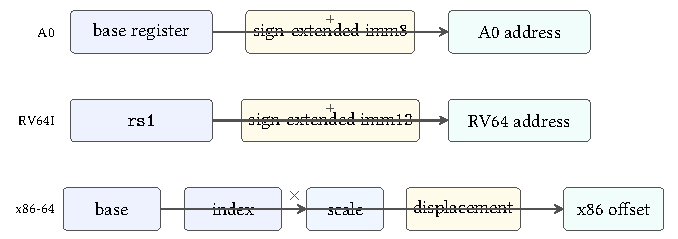
\includegraphics[width=0.98\textwidth]{figures/effective-addresses}
\caption{Selected effective-address shapes. A0 and RV64I use one base and a
sign-extended immediate. A selected x86-64 form can combine base, scaled index,
and displacement. Every result still needs a validity check before access.}
\figalt{Three rows compare base plus immediate for A0, rs1 plus immediate for RV64I, and base plus index times scale plus displacement for x86-64.}
\label{fig:effective-addresses}
\end{figure}

A0 and the selected RV64I loads share the broad equation
\[
  a=\mathit{base}+\mathit{signExtendedOffset}\pmod {2^{64}}
\]
when A0 is instantiated at width 64. The immediate widths differ: eight bits
for A0 and twelve bits for the selected RV64I form. Their encodings and failure
environments also differ.

A selected x86-64 memory operand can compute
\[
  a=\mathit{base}+s\cdot\mathit{index}+\mathit{displacement}
       \pmod {2^{64}},
\]
where the scale \(s\) is 1, 2, 4, or 8. A form need not use every component.
The encoding can omit a base, omit an index, or use instruction-pointer-relative
addressing. This chapter initially uses the ordinary 64-bit address size and a
flat address space without nonzero FS or GS bases. Intel's current basic
architecture manual supplies the complete mode-dependent rules
\autocite{intel2026sdm1}.

Suppose \code{rbx=0x1000}, \code{rcx=3}, the scale is 8, and the displacement
is 16. The selected x86-64 address is
\[
  \mathtt{1000}+3\mathbin{\cdot}8+16=\mathtt{1028}.
\]
The scale naturally matches an eight-byte array element, while the displacement
can locate a field within or beyond the indexed object. The hardware does not
know that story. It performs the declared arithmetic and access checks.

\begin{warning}[title={Address arithmetic is not an object-bounds proof}]
An effective address can be numerically valid while pointing outside the
programmer's intended array or object. The ISA supplies address arithmetic and
architectural faults. Language-level provenance and object bounds require
additional models and premises.
\end{warning}

Address wrapping and range validity are distinct. If the word-sized addition
wraps, the resulting address may still fall inside the finite modeled memory.
A theorem that intends to exclude wrap must say so as a precondition. Merely
checking the final byte range does not establish that the mathematical sum fit.

\subsection{Address formation and memory access are separate stages}

A load or store proof is clearer when decomposed into stages. First read every
old operand needed for the source and address. Next calculate the effective
address as a word. Then check the complete byte range and any selected
alignment, permission, or address-validity policy. Only after those checks does
a load assemble bytes or a store split its source into bytes. Finally, commit
one successor state or one declared failure outcome.

\begin{figure}[htbp]
\centering
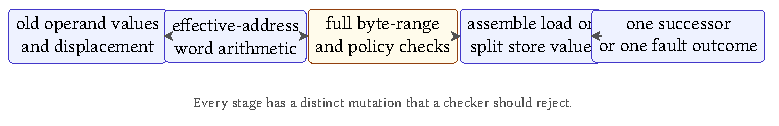
\includegraphics[width=0.98\textwidth]{figures/memory-transfer-gates}
\caption{A memory transfer crosses several semantic gates. Separating them
makes failure ordering, preservation, and negative controls explicit.}
\figalt{Old operands lead to effective-address arithmetic, full byte-range and policy checks, load assembly or store splitting, and a committed successor or fault.}
\label{fig:memory-transfer-gates}
\end{figure}

This order prevents self-dependence errors. In a load whose destination
register also supplies the base, the address uses the old register value.
Likewise, a store reads its source word before updating any overlapping memory
byte in the atomic architectural step. A functional state update naturally
expresses this order when all right-hand sides are evaluated from the entry
state.

Range checking must include width. For an \(n\)-byte access at word address
\(a\), the intended mathematical interval is \([a,a+n)\). Under a finite
word address model, proving that interval valid requires more than checking
\(a+n-1\) after modular arithmetic. The addition might wrap to a small final
address. One safe premise is
\[
  \langle a\rangle_u+n\leq 2^w
\]
together with membership of every address in the modeled readable or writable
region.

\begin{proofkit}[title={Full-range validity from endpoint inequalities}]
Assume ordinary address arithmetic does not wrap, and a permitted memory
region is the half-open interval \([b,e)\). An \(n\)-byte access beginning
at \(a\) lies inside it exactly when \(b\leq a\) and \(a+n\leq e\).
The first inequality protects the low endpoint. The second protects every byte
through \(a+n-1\). Half-open intervals make an access ending exactly at
\(e\) valid without admitting byte \(e\).
\end{proofkit}

Alignment is another policy, not a consequence of range validity. An eight-
byte access at address 3 can lie wholly within mapped memory while failing a
model that requires divisibility by eight. Other selected environments may
permit the access, split it internally, or report a different failure. A
machine-code theorem must pin the policy actually used rather than infer it
from the operand width.

\begin{warning}[title={Do not merge all memory failures}]
An out-of-range address, an alignment violation, a permission failure, and a
later translation fault can preserve the same destination while arising at
different stages. If the model distinguishes them or their priority, the
trace and refinement relation must distinguish them too.
\end{warning}

\section{RV64I movement: widths are in the instruction}

Our RV64I window uses the base integer ISA at XLEN 64. Register \code{x0}
always reads as zero, and writes to it have no architectural effect. The other
31 integer registers hold 64-bit words. Loads and stores form addresses by
adding a sign-extended 12-bit immediate to \code{rs1}
\autocite{riscv2026unpriv}.

\code{ld x5,16(x6)} reads eight bytes at \code{x6+16}, assembles a 64-bit
little-endian word, and writes it to \code{x5}. \code{sd x5,16(x6)} writes
the low 64 bits of \code{x5} to the same byte range. These are the closest
selected counterparts to width-64 A0 load and store.

Narrow loads make the value rule visible. \code{lw} loads four bytes and
sign-extends bit 31 through the 64-bit destination. \code{lwu} loads the same
four bytes and fills bits 63--32 with zeros. Likewise, \code{lb} and
\code{lbu} differ only in how they form the high 56 destination bits; the
memory range and low byte can be identical.

Stores do not extend. \code{sb}, \code{sh}, and \code{sw} write the low 8,
16, or 32 bits of \code{rs2}. The high source bits are ignored for that
access. Neighboring bytes outside the selected range remain unchanged.

\begin{example}[title={One RV64 word load, two destination values}]
Let bytes at addresses \(a\) through \(a+3\) be \code{00 00 00 80}.
Little-endian assembly gives the 32-bit word \code{80000000}. An \code{lw}
produces \code{FFFFFFFF80000000}; an \code{lwu} produces
\code{0000000080000000}. Both read the same bytes. The instruction's extension
rule creates the difference.
\end{example}

\subsection{Extension is a theorem about all destination bits}

Let \(u\) be the unsigned reading of an \(n\)-bit source and let the
destination width be \(m>n\). Zero extension preserves the same nonnegative
reading:
\[
  \langle\mathsf{zext}_{m}(x)\rangle_u=u.
\]
Sign extension instead preserves the source's signed two's-complement reading.
If the source high bit is zero, both extensions agree. If it is one, sign
extension fills the new high bits with ones while zero extension fills them
with zeros.

This gives an exact agreement condition useful in optimization proofs:
\[
  \mathsf{zext}_{m}(x)=\mathsf{sext}_{m}(x)
  \quad\hbox{iff}\quad \mathrm{bit}_{n-1}(x)=0.
\]
The forward direction follows because the new high bits differ when the source
high bit is one. The reverse direction follows because both operations then
copy the low \(n\) bits and fill every new bit with zero.

\begin{proofkit}[title={A narrow load has two independent obligations}]
First prove that the instruction reads exactly the selected \(n/8\) bytes and
assembles the intended source word in the declared byte order. Then prove that
its extension rule forms the full \(m\)-bit destination. Matching the low
source bits does not discharge the high-bit obligation, and matching the final
word does not by itself prove that the correct memory interval was read.
\end{proofkit}

Narrow stores have the dual shape but no extension. They select the low source
bits, split them according to byte order, and update exactly the destination
interval. A round trip through a narrow store and wider sign-extending load
does not generally recover the original wide register; it recovers the signed
extension of the stored low portion.

An immediate arithmetic instruction can also serve movement. \code{addi x5,x6,0}
copies \code{x6} to \code{x5} as an assembler pseudoinstruction commonly
spelled \code{mv x5,x6}. The hardware-visible instruction is still ADDI. If
the destination is \code{x0}, the calculated result is discarded. Decoding must
retain \code{rd=0}; execution enforces the special destination behavior.

\begin{sidebar}[title={Pseudoinstructions belong to the notation layer}]
A pseudoinstruction can make source code easier to read without adding an ISA
operation. Proof artifacts should record the decoded base instruction and its
operands. The chapter may print the convenient spelling beside it, but should
not count the alias as another machine instruction.
\end{sidebar}

\section{x86-64 movement: register names carry width}

x86-64 names overlapping portions of a general-purpose register. In the RAX
family, \code{rax} names 64 bits, \code{eax} the low 32, \code{ax} the low
16, and \code{al} the low 8. These are not four independent storage cells.
The destination name and instruction form determine what happens to the whole
architectural register.

In 64-bit mode, a 32-bit write to a general-purpose register zeros its upper
32 bits. Thus \code{mov eax,ebx} writes the low 32 bits from EBX and leaves
RAX with a zero high half. A 16-bit write to AX or an 8-bit write to AL does
not receive that automatic full-register zeroing rule; the unselected higher
bits of RAX remain as specified by the instruction form.

\begin{figure}[htbp]
\centering
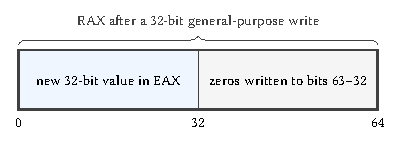
\includegraphics[width=0.92\textwidth]{figures/x64-subregister-write}
\caption{A selected 32-bit general-purpose destination write in 64-bit mode
defines all 64 bits of the containing register: the high half becomes zero.}
\figalt{A 64-bit RAX bar shows a new value in low bits 0 through 31 and zeros written to bits 32 through 63.}
\label{fig:x64-subregister-write}
\end{figure}

Let RAX initially be \code{1122334455667788}. After writing \code{AABBCCDD}
to EAX, RAX is \code{00000000AABBCCDD}. After instead writing \code{EEFF}
to AX, RAX is \code{112233445566EEFF}. A proof that observes only the named
destination width misses the difference in the containing register.

x86-64 also distinguishes moves that extend a smaller source. A selected
zero-extending move fills the new high bits with zero; a selected sign-extending
move copies the narrow sign bit. Ordinary MOV between equal-width register or
memory operands does neither. The exact opcode and operand sizes must be named
before the word ``move'' has a complete value rule. The pinned Intel instruction
reference provides those form-specific contracts \autocite{intel2026sdm2}.

The LEA instruction is a useful boundary case. For a selected 64-bit form, it
computes the offset described by a memory-style addressing expression and
writes that number to a register. It does not read the memory bytes at that
address. Therefore a bad pointer can be harmless under LEA and fault under a
MOV load that uses the same printed brackets.

\begin{tryit}[title={Address calculation is not memory movement}]
Choose base, index, scale, and displacement so the calculated offset lies outside
the chapter's valid memory. Compare a selected LEA-like address computation
with a load from that address. The first can still produce the numeric word;
the second must pass an access check before writing its destination.
\end{tryit}

Instruction-pointer-relative addressing adds a timing detail to the address
equation. In a selected x86-64 form, the base is the address following the
instruction, not its first byte. Because instruction length is determined by
decode, address formation depends on faithful length decoding. Relocating the
instruction and its referenced object together can preserve the displacement,
but changing the encoding length at the same address changes the base and may
require displacement repair.

The scale field also has limits. It multiplies the index by 1, 2, 4, or 8; it
does not encode an arbitrary element size. An array of 12-byte records may
need an earlier arithmetic instruction or a combination such as three times an
index followed by scale four. The effective-address theorem should describe
the actual arithmetic sequence rather than attribute source-level array
semantics to one addressing form.

\begin{sidebar}[title={An address expression has no inherent object type}]
The same base-plus-index expression can locate an array element, a structure
field, a table entry, or bytes outside every intended object. Machine semantics
provides the numeric word and access behavior. Object identity and provenance
enter only through a stronger language or compiler relation.
\end{sidebar}

\section{Relating selected movements}

A real instruction refines an A0 movement when related starting states lead
to related results under printed preconditions. The relation can translate
register names and instruction addresses. It cannot discard a destination-width
effect that a later observation can reveal.

For width-64 A0 load and RV64I \code{ld}, a simple relation can map one A0
register to \code{rs1}, another to \code{rd}, and equate their finite memory
windows byte for byte. The immediate relation must equate A0's sign-extended
eight-bit offset with RV64I's sign-extended twelve-bit offset for the selected
values. Both accesses must be valid. The post-relation equates destination
words, preserved memory, running outcomes, and logical successor positions.

The same direct relation does not cover \code{lw}. A0's width-64 load reads
eight bytes, while \code{lw} reads four and sign-extends. We can instead use
a width-32 A0 instance and add an explicit sign-extension bridge, or define a
more abstract operation that reads four bytes and produces a 64-bit extended
result. The model should change visibly rather than pretending the widths match.

For x86-64 \code{mov eax,ebx}, an A0 width-32 move can match the low result.
To relate full 64-bit states, the bridge must also require the x86 destination's
upper half to be zero after the step. If the A0 state has only 32-bit registers,
that fact may live in a representation invariant rather than a destination
equality.

\begin{warning}[title={Fault agreement is part of movement refinement}]
Two instructions do not refine the same operation merely because their
successful destination values agree. If one can trap on an address where the
other succeeds, either exclude that input, relate the fault outcomes, or weaken
the claim. Silently comparing only successful runs changes the theorem.
\end{warning}

Aliasing adds another premise. Suppose the destination register contributes to
the address. An architectural instruction reads the old operand values needed
for its address and source before committing the destination write. A symbolic
implementation that updates the register first can compute the address from
the new value and still look plausible on non-aliasing tests. Read sets and
write order should be explicit even when the mathematical transition is
presented as one atomic step.

\subsection{When two memory movements may commute}

Reordering independent loads and stores is central to compilers and processors,
but independence is a semantic claim. Two stores to disjoint byte intervals
commute in this chapter's atomic memory model when both addresses and source
values are already fixed by state neither store changes. Applying either store
first yields the same final byte map because each update preserves every byte
written by the other.

Overlap breaks the argument. If one store writes \([a,a+4)\) and another
writes \([a+2,a+6)\), their final values at bytes \(a+2\) and \(a+3\)
depend on order. A load and store also fail to commute when the load reads a
byte the store changes. Even disjoint memory intervals are insufficient if a
destination register of the first load supplies the second instruction's
address.

\begin{proofkit}[title={Disjoint stores commute}]
Let store \(A\) update interval \(I\) with byte function \(v_A\), and store
\(B\) update disjoint interval \(J\) with \(v_B\). Consider an arbitrary
address \(q\). If \(q\in I\), both orders leave \(v_A(q)\) because
\(q\notin J\). If \(q\in J\), both leave \(v_B(q)\). Outside
\(I\cup J\), both preserve the entry byte. The final memories are therefore
equal pointwise. The argument also requires both steps to have the same
successful outcomes in either order.
\end{proofkit}

Faults make the last sentence load-bearing. Suppose the first store succeeds
and the second faults. In an architecture with one committed instruction per
step, swapping them changes whether the first store becomes visible before the
fault. A refinement that observes only final successful runs hides this
difference. Reordering needs a premise that both accesses succeed, or a richer
argument about permitted fault behavior.

The same footprint reasoning explains why a single x86-64 memory-source
arithmetic instruction cannot always be replaced by a load followed by
register arithmetic. The expanded sequence introduces an intermediate state
and perhaps a different fault boundary. Under a no-fault premise and an
observation only at the sequence endpoints, the replacement may still be
valid; without those conditions, instruction count is not the only change.

\section{How Axeyum enters this chapter}

The live Axeyum checkout still lacks A0, RV64I, and x86-64 architectural
packages. This chapter therefore defines the first data-movement obligations
rather than reporting completed machine proofs.

Start with an executable A0 transfer package. Represent the register map,
finite byte memory, and running/trapped outcome. Implement \code{mov},
\code{movi}, \code{load}, and \code{store}. Reuse Axeyum's bit-vector
machinery for extension, truncation, word addition, and byte extraction. Every
operation should return a complete successor state rather than only its main
result.

The smallest useful property family includes immediate sign extension,
store-then-load reconstruction, preservation of untouched registers and bytes,
range failure without partial writes, and wrapped-address controls. Run small
widths exhaustively where possible. Use solver search at larger widths, but
replay any model through the executable transition.

Then add thin adapters for the selected real forms. The RV64 adapter needs
\code{x0}, 12-bit offsets, narrow load extension, and narrow stores. The
x86-64 adapter needs selected subregister writes and the chosen effective-address
form. Each adapter should name its manual revision and refuse every form outside
its declared slice.

Build the checker around the staged pipeline in
Figure~\ref{fig:memory-transfer-gates}. Record the old operands separately
from the effective address so a mutation that substitutes the new destination
value can be detected. Record the requested width and full interval so a
first-byte-only range check cannot pass. Reconstruct loaded values and store
bytes inside the checker rather than trusting either derived field in the
artifact.

The initial control set should change one fact at a time: immediate sign
extension, address wrap, access width, byte order, load extension, store
truncation, x86 subregister preservation, and fault atomicity. Each control
needs a small witness whose failure class is known in advance. That structure
turns an Axeyum example into a lesson about the contract rather than a single
opaque pass result.

\begin{goingdeeper}[title={A good first solver question}]
Ask whether zero-extending and sign-extending an \(n\)-bit value to a wider
word ever agree when the source high bit is one. The solver should report no
such value. Flip the premise to high bit zero and prove they always agree. The
pair tests extension definitions, premise handling, and the negative-control
route before any full instruction semantics depends on them.
\end{goingdeeper}

An artifact for this chapter will eventually record inputs, initial memory,
decoded instruction, calculated effective address, bytes read or written, full
successor state, source pins, Axeyum revision, and control results. Until such
an artifact is active, the examples remain reader-checkable specification work.

\section{Where the model stops}

This chapter uses finite byte memory and single-threaded atomic instruction
steps. It does not model caches, translation lookaside buffers, page tables,
weak memory, concurrency, memory-mapped devices, or speculative execution. It
does not claim the full RV64I or x86-64 addressing repertoire.

The x86-64 discussion assumes ordinary 64-bit address size and a flat segment
base for the selected examples. The RV64I discussion leaves access-fault and
misalignment policy to a later execution-environment pin where the base
unprivileged ISA does. These limits are not footnotes to the theorem. They say
which machine the theorem is about.

Within that machine, something broad has become exact. A0, RV64I, and x86-64
can spell movement differently, yet the comparison reduces to finite words,
named locations, address equations, byte ranges, and observations. Once those
objects are written down, resemblance can give way to a relation that either
holds or produces a counterexample.

The durable lesson is to resist treating movement as the easy part between
interesting calculations. A value has a width and interpretation; a location
has a footprint; an address has an arithmetic derivation; an access has a
range and failure policy; and a destination write has a rule for the rest of
its containing storage. Those facts determine whether later arithmetic and
control flow receive the state the programmer intended.

This decomposition also gives a practical proof order. Establish operand
reads, calculate the address, justify the complete access, construct the
destination value, and finally prove preservation. When a witness disagrees,
the failed layer tells the reader what kind of movement error occurred.

\section{Exercises}

\begin{enumerate}
\item \textbf{Execute.} At A0 width 16, trace \code{movi r2,0x80}. Give the
complete destination word, next program counter, preserved state, and outcome.

\item Trace a width-16 A0 store followed by a load at the same address. List
the two bytes after the store and reconstruct the loaded word.

\item \textbf{Break.} Change the A0 load implementation so it checks only
the first byte of the range. Construct a final-address example that exposes a
partial or out-of-range read.

\item Give an eight-bit source for which zero extension and sign extension to
64 bits differ. Give a second source for which they agree, and explain why.

\item Compute the selected x86-64 effective address for base \code{0x2000},
index 5, scale 4, and displacement -8. Show the word arithmetic before any
memory validity decision.

\item Starting from RAX \code{FFEEDDCCBBAA9988}, compute full RAX after
writing \code{12345678} to EAX, \code{1234} to AX, and \code{12} to AL in
three separate initial states.

\item Compare RV64I \code{lw} and \code{lwu} on bytes
\code{FF FF FF FF}. Construct one observation that distinguishes the results
and one that does not.

\item Explain why \code{addi x5,x6,0} may be printed as a move while its
decoded instruction remains ADDI. What should an evidence manifest record?

\item \textbf{Prove.} State and prove the preservation clauses for an A0
register move. Include the case where source and destination are equal.

\item Prove that two disjoint A0 stores commute under the chapter's atomic
memory model. Identify the premise that fails when the byte ranges overlap.

\item \textbf{Transfer.} Write a state relation for one width-64 A0 load and
RV64I \code{ld}. Name the register map, memory agreement, offset condition,
validity premise, and post-state observation.

\item Extend that relation to a selected x86-64 load using base plus scaled
index plus displacement. State which address-size and segment assumptions are
required.

\item Design an Axeyum negative control that changes sign extension to zero
extension. Give one concrete witness it must find and the failure class the
checker should report.
\end{enumerate}
